\documentclass[12pt]{article}\usepackage[]{graphicx}\usepackage[]{color}
%% maxwidth is the original width if it is less than linewidth
%% otherwise use linewidth (to make sure the graphics do not exceed the margin)
\makeatletter
\def\maxwidth{ %
  \ifdim\Gin@nat@width>\linewidth
    \linewidth
  \else
    \Gin@nat@width
  \fi
}
\makeatother

\definecolor{fgcolor}{rgb}{0.345, 0.345, 0.345}
\newcommand{\hlnum}[1]{\textcolor[rgb]{0.686,0.059,0.569}{#1}}%
\newcommand{\hlstr}[1]{\textcolor[rgb]{0.192,0.494,0.8}{#1}}%
\newcommand{\hlcom}[1]{\textcolor[rgb]{0.678,0.584,0.686}{\textit{#1}}}%
\newcommand{\hlopt}[1]{\textcolor[rgb]{0,0,0}{#1}}%
\newcommand{\hlstd}[1]{\textcolor[rgb]{0.345,0.345,0.345}{#1}}%
\newcommand{\hlkwa}[1]{\textcolor[rgb]{0.161,0.373,0.58}{\textbf{#1}}}%
\newcommand{\hlkwb}[1]{\textcolor[rgb]{0.69,0.353,0.396}{#1}}%
\newcommand{\hlkwc}[1]{\textcolor[rgb]{0.333,0.667,0.333}{#1}}%
\newcommand{\hlkwd}[1]{\textcolor[rgb]{0.737,0.353,0.396}{\textbf{#1}}}%

\usepackage{framed}
\makeatletter
\newenvironment{kframe}{%
 \def\at@end@of@kframe{}%
 \ifinner\ifhmode%
  \def\at@end@of@kframe{\end{minipage}}%
  \begin{minipage}{\columnwidth}%
 \fi\fi%
 \def\FrameCommand##1{\hskip\@totalleftmargin \hskip-\fboxsep
 \colorbox{shadecolor}{##1}\hskip-\fboxsep
     % There is no \\@totalrightmargin, so:
     \hskip-\linewidth \hskip-\@totalleftmargin \hskip\columnwidth}%
 \MakeFramed {\advance\hsize-\width
   \@totalleftmargin\z@ \linewidth\hsize
   \@setminipage}}%
 {\par\unskip\endMakeFramed%
 \at@end@of@kframe}
\makeatother

\definecolor{shadecolor}{rgb}{.97, .97, .97}
\definecolor{messagecolor}{rgb}{0, 0, 0}
\definecolor{warningcolor}{rgb}{1, 0, 1}
\definecolor{errorcolor}{rgb}{1, 0, 0}
\newenvironment{knitrout}{}{} % an empty environment to be redefined in TeX

\usepackage{alltt}

\usepackage{amssymb,amsmath}
\usepackage{enumerate}
\usepackage{verbatim}
\usepackage{graphicx, multicol}
\usepackage{float}

%% LaTeX margin settings:
  \setlength{\textwidth}{7.0in}
\setlength{\textheight}{9in}
\setlength{\oddsidemargin}{-.5in}
\setlength{\evensidemargin}{0in}
\setlength{\topmargin}{-1.5cm}

%% tell knitr to use smaller font for code chunks
\def\fs{\footnotesize}
\def\R{{\sf R}}
\newcommand{\bfbeta}{\mbox{\boldmath $\beta$}}
\newcommand{\bfD}{\mbox{\boldmath $D$}}
\newcommand{\bfL}{\mbox{\boldmath $L$}}
\newcommand{\bfR}{\mbox{\boldmath $R$}}
\newcommand{\bfmu}{\mbox{\boldmath $\mu$}}
\newcommand{\bfv}{\mbox{\boldmath $V$}}
\newcommand{\bfX}{\mbox{\boldmath $X$}}
\newcommand{\bfy}{\mbox{\boldmath $y$}}
\newcommand{\bfb}{\mbox{\boldmath $b$}}
\IfFileExists{upquote.sty}{\usepackage{upquote}}{}
\begin{document}



  
  
\begin{center}
\large{Bayes Midterm 2} \\
Leslie Gains-Germain
\end{center}

\begin{enumerate}

\item \begin{enumerate}

\item The following example was inspired by Claire and Jordan's consulting project. Suppose there are five reservations in Montana. The number of children eligible to receive dental sealants on the reservation is unknown because it's hard to keep track of this population. A success is observed when a child comes to a dental clinic to have dental sealants applied. The number of children on each of the five reservations who had dental sealants applied in $2014$ was observed. The probability of having the sealants applied and the number of eligible children is assumed to be the same for all five reservations. 

\item The MLE occurs near $m=101, \pi=0.21$. 

\begin{knitrout}\footnotesize
\definecolor{shadecolor}{rgb}{0.969, 0.969, 0.969}\color{fgcolor}
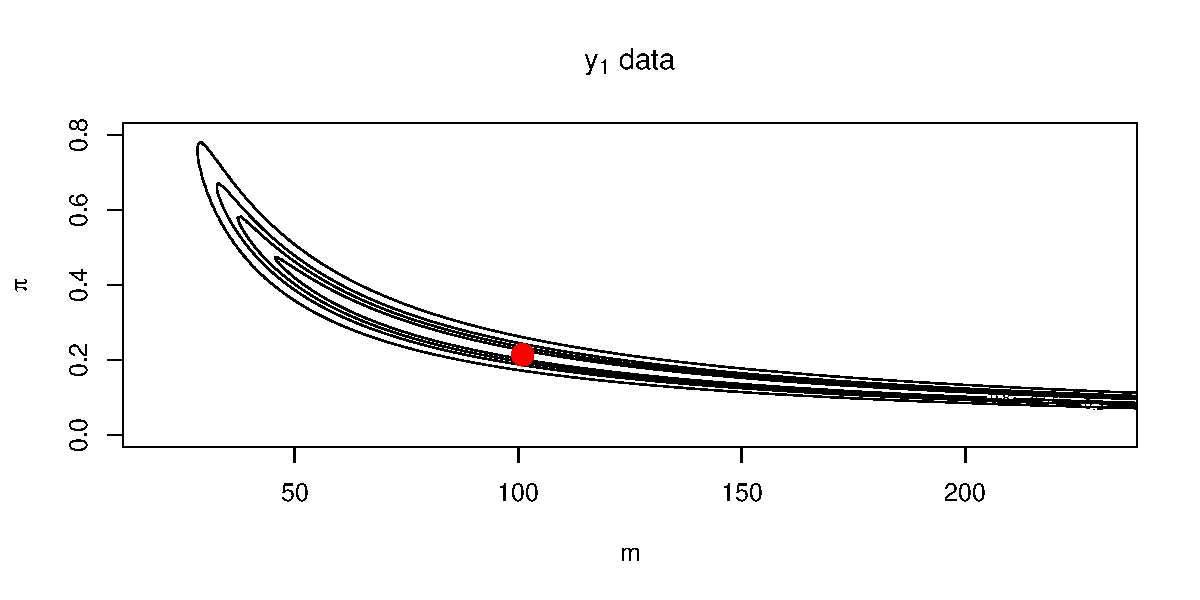
\includegraphics[width=\linewidth]{figure/likelihood-1} 

\end{knitrout}

\item The MLE occurs near $m=196, \pi=0.11$. 

\begin{knitrout}\footnotesize
\definecolor{shadecolor}{rgb}{0.969, 0.969, 0.969}\color{fgcolor}
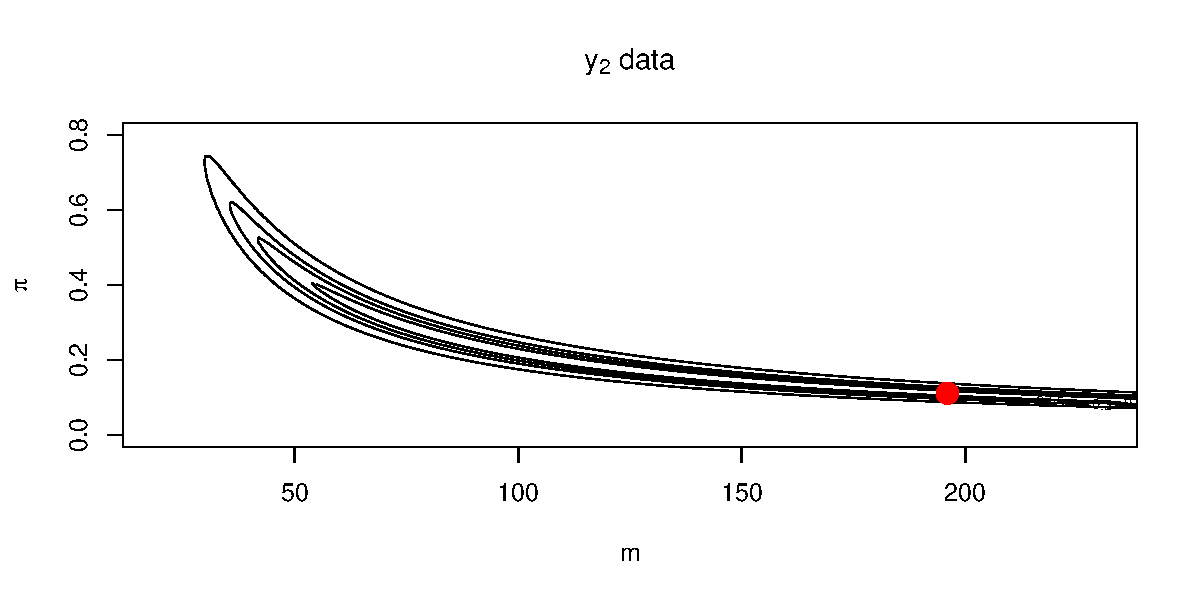
\includegraphics[width=\linewidth]{figure/likelihood2-1} 

\end{knitrout}

\item \begin{enumerate}

\item The joint posterior distribution of $(m, \pi)$ is shown below.

\begin{knitrout}\footnotesize
\definecolor{shadecolor}{rgb}{0.969, 0.969, 0.969}\color{fgcolor}
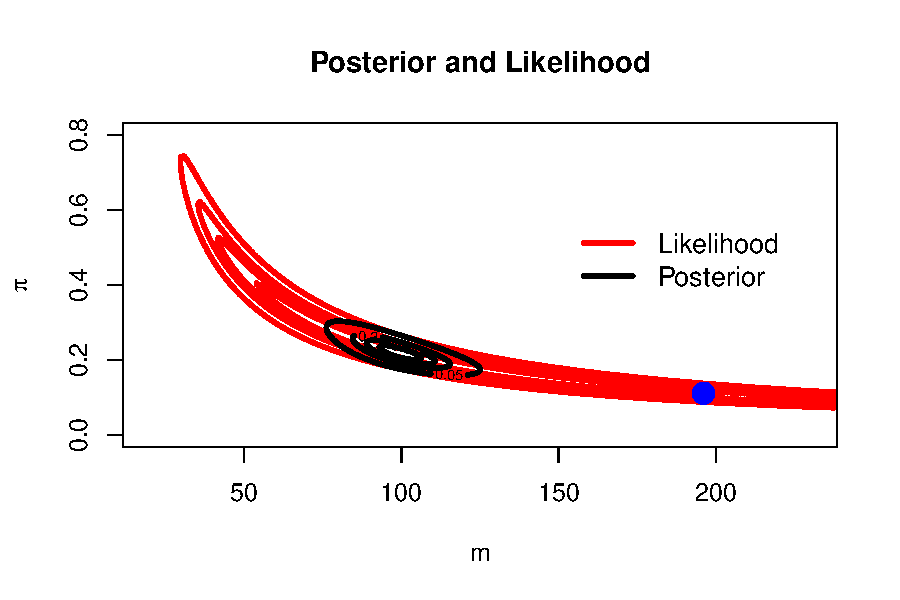
\includegraphics[width=\linewidth]{figure/jointpost-1} 

\end{knitrout}

\item My work for deriving the complete conditionals for $m$ and $\pi$ is shown below.
\begin{align*}
p(\pi|y, m) &= \frac{p(\pi, y, m)}{p(y, m)} \\
&\propto p(\pi, y, m) \\
&\propto p(y|\pi, m)p(m, \pi) \\
&\propto p(y|\pi, m)p(\pi) \\
p(m|y, \pi) &= \frac{p(\pi, y, m)}{p(y, \pi)} \\
&\propto p(\pi, y, m) \\
&\propto p(y|\pi, m)p(m, \pi) \\
&\propto p(y|\pi, m)p(m)
\end{align*}

\item My code for the Gibbs sampler is shown below.

\begin{knitrout}\footnotesize
\definecolor{shadecolor}{rgb}{0.969, 0.969, 0.969}\color{fgcolor}\begin{kframe}
\begin{alltt}
\hlcom{#function to calculate complete conditional for pi on log scale}
\hlstd{log.pi.cc.fun} \hlkwb{<-} \hlkwa{function}\hlstd{(}\hlkwc{m.pi}\hlstd{,} \hlkwc{y.vec}\hlstd{)\{}
  \hlkwd{loglik.fun}\hlstd{(m.pi, y.vec)}
\hlstd{\}}

\hlcom{#check function}
\hlcom{#log.pi.cc.fun(c(40, 0.5), y2.data)}

\hlcom{#function to calculate complete conditional for m on log scale}
\hlstd{log.m.cc.fun} \hlkwb{<-} \hlkwa{function}\hlstd{(}\hlkwc{m.pi}\hlstd{,} \hlkwc{y.vec}\hlstd{)\{}
  \hlkwd{log.post.fun}\hlstd{(m.pi, y.vec)}
\hlstd{\}}

\hlcom{#check function}
\hlcom{#log.m.cc.fun(c(40, 0.5), y2.data)}

\hlstd{nchain} \hlkwb{<-} \hlnum{3}
\hlstd{nsim} \hlkwb{<-} \hlnum{10000}
\hlstd{m.pi.mat} \hlkwb{<-} \hlkwd{array}\hlstd{(}\hlnum{NA}\hlstd{,} \hlkwc{dim}\hlstd{=}\hlkwd{c}\hlstd{(nsim,} \hlnum{2}\hlstd{, nchain))}

\hlcom{#keep track of acceptance ratios}
\hlstd{jump.mat} \hlkwb{<-} \hlkwd{matrix}\hlstd{(}\hlnum{NA}\hlstd{,} \hlkwc{nrow}\hlstd{=nsim}\hlopt{-}\hlnum{1}\hlstd{,} \hlkwc{ncol}\hlstd{=}\hlnum{2}\hlstd{)}

\hlcom{#specify starting values for each chain}
\hlstd{m.pi.mat[}\hlnum{1}\hlstd{,} \hlnum{1}\hlopt{:}\hlnum{2}\hlstd{,} \hlnum{1}\hlstd{]} \hlkwb{<-} \hlkwd{c}\hlstd{(}\hlnum{100}\hlstd{,} \hlnum{0.4}\hlstd{)}
\hlstd{m.pi.mat[}\hlnum{1}\hlstd{,} \hlnum{1}\hlopt{:}\hlnum{2}\hlstd{,} \hlnum{2}\hlstd{]} \hlkwb{<-} \hlkwd{c}\hlstd{(}\hlnum{50}\hlstd{,} \hlnum{0.2}\hlstd{)}
\hlstd{m.pi.mat[}\hlnum{1}\hlstd{,} \hlnum{1}\hlopt{:}\hlnum{2}\hlstd{,} \hlnum{3}\hlstd{]} \hlkwb{<-} \hlkwd{c}\hlstd{(}\hlnum{150}\hlstd{,} \hlnum{0.4}\hlstd{)}

\hlcom{#define standard deviations for normal proposal distributions}
\hlstd{sd.scale} \hlkwb{<-} \hlkwd{c}\hlstd{(}\hlnum{10}\hlstd{,} \hlnum{5}\hlstd{)}

\hlkwd{set.seed}\hlstd{(}\hlnum{230923}\hlstd{)}

\hlkwa{for} \hlstd{(j} \hlkwa{in} \hlnum{1}\hlopt{:}\hlstd{nchain) \{}
  \hlkwa{for} \hlstd{(i} \hlkwa{in} \hlnum{2}\hlopt{:}\hlstd{nsim) \{}
    \hlcom{#set pi equal to the starting value}
    \hlstd{pi} \hlkwb{<-} \hlstd{m.pi.mat[i}\hlopt{-}\hlnum{1}\hlstd{,} \hlnum{2}\hlstd{, j]}

    \hlcom{#now draw m from complete conditional with Metropolis Hastings Algorithm}
    \hlstd{m.cur} \hlkwb{<-} \hlstd{m.pi.mat[i}\hlopt{-}\hlnum{1}\hlstd{,} \hlnum{1}\hlstd{, j]}
    \hlstd{m.cand} \hlkwb{<-} \hlkwd{rpois}\hlstd{(}\hlnum{1}\hlstd{,} \hlkwc{lambda}\hlstd{=m.cur)}

    \hlstd{log.r.num.m} \hlkwb{<-} \hlkwd{log.m.cc.fun}\hlstd{(}\hlkwd{c}\hlstd{(m.cand, pi),} \hlkwc{y.vec} \hlstd{= y2.data)} \hlopt{+}
                     \hlkwd{dpois}\hlstd{(m.cur,} \hlkwc{lambda}\hlstd{=m.cand,} \hlkwc{log} \hlstd{=} \hlnum{TRUE}\hlstd{)}

    \hlstd{log.r.denom.m} \hlkwb{<-} \hlkwd{log.m.cc.fun}\hlstd{(}\hlkwd{c}\hlstd{(m.cur, pi),} \hlkwc{y.vec} \hlstd{= y2.data)} \hlopt{+}
                       \hlkwd{dpois}\hlstd{(m.cand,} \hlkwc{lambda}\hlstd{=m.cur,} \hlkwc{log} \hlstd{=} \hlnum{TRUE}\hlstd{)}

    \hlstd{log.r.m} \hlkwb{<-} \hlstd{log.r.num.m} \hlopt{-} \hlstd{log.r.denom.m}

    \hlstd{p.accept.m} \hlkwb{<-} \hlkwd{min}\hlstd{(}\hlnum{1}\hlstd{,} \hlkwd{exp}\hlstd{(log.r.m))}

    \hlstd{u.vec} \hlkwb{<-} \hlkwd{runif}\hlstd{(}\hlnum{2}\hlstd{)}

    \hlkwd{ifelse}\hlstd{(u.vec[}\hlnum{1}\hlstd{]} \hlopt{<=} \hlstd{p.accept.m, m.pi.mat[i,} \hlnum{1}\hlstd{, j]} \hlkwb{<-} \hlstd{m.cand,}
           \hlstd{m.pi.mat[i,} \hlnum{1}\hlstd{, j]} \hlkwb{<-} \hlstd{m.cur)}

    \hlstd{jump.mat[i}\hlopt{-}\hlnum{1}\hlstd{,} \hlnum{1}\hlstd{]} \hlkwb{<-} \hlkwd{ifelse}\hlstd{(u.vec[}\hlnum{1}\hlstd{]} \hlopt{<=} \hlstd{p.accept.m,} \hlnum{1}\hlstd{,} \hlnum{0}\hlstd{)}

    \hlcom{#now fix m at its value in the ith iteration}
    \hlstd{m} \hlkwb{<-} \hlstd{m.pi.mat[i,} \hlnum{1}\hlstd{, j]}

    \hlcom{#draw pi from complete conditional with metropolis hastings algorithm}
    \hlstd{pi.cur} \hlkwb{<-} \hlstd{m.pi.mat[i}\hlopt{-}\hlnum{1}\hlstd{,} \hlnum{2}\hlstd{, j]}
    \hlstd{pi.cand} \hlkwb{<-} \hlkwd{rbeta}\hlstd{(}\hlnum{1}\hlstd{,} \hlnum{2}\hlstd{, sd.scale[}\hlnum{2}\hlstd{])}

    \hlstd{log.r.num.pi} \hlkwb{<-} \hlkwd{log.pi.cc.fun}\hlstd{(}\hlkwd{c}\hlstd{(m, pi.cand),} \hlkwc{y.vec} \hlstd{= y2.data)} \hlopt{+}
                     \hlkwd{dbeta}\hlstd{(pi.cur,} \hlnum{2}\hlstd{, sd.scale[}\hlnum{2}\hlstd{],} \hlkwc{log} \hlstd{=} \hlnum{TRUE}\hlstd{)}

    \hlstd{log.r.denom.pi} \hlkwb{<-} \hlkwd{log.pi.cc.fun}\hlstd{(}\hlkwd{c}\hlstd{(m, pi.cur),} \hlkwc{y.vec} \hlstd{= y2.data)} \hlopt{+}
                       \hlkwd{dbeta}\hlstd{(pi.cand,} \hlnum{2}\hlstd{, sd.scale[}\hlnum{2}\hlstd{],} \hlkwc{log} \hlstd{=} \hlnum{TRUE}\hlstd{)}

    \hlstd{log.r.pi} \hlkwb{<-} \hlstd{log.r.num.pi} \hlopt{-} \hlstd{log.r.denom.pi}

    \hlstd{p.accept.pi} \hlkwb{<-} \hlkwd{min}\hlstd{(}\hlnum{1}\hlstd{,} \hlkwd{exp}\hlstd{(log.r.pi))}

    \hlstd{u.vec} \hlkwb{<-} \hlkwd{runif}\hlstd{(}\hlnum{2}\hlstd{)}

    \hlkwd{ifelse}\hlstd{(u.vec[}\hlnum{2}\hlstd{]} \hlopt{<=} \hlstd{p.accept.pi, m.pi.mat[i,} \hlnum{2}\hlstd{, j]} \hlkwb{<-} \hlstd{pi.cand,}
           \hlstd{m.pi.mat[i,} \hlnum{2}\hlstd{, j]} \hlkwb{<-} \hlstd{pi.cur)}

    \hlstd{jump.mat[i}\hlopt{-}\hlnum{1}\hlstd{,} \hlnum{2}\hlstd{]} \hlkwb{<-} \hlkwd{ifelse}\hlstd{(u.vec[}\hlnum{2}\hlstd{]} \hlopt{<=} \hlstd{p.accept.pi,} \hlnum{1}\hlstd{,} \hlnum{0}\hlstd{)}
  \hlstd{\}}
\hlstd{\}}
\end{alltt}
\end{kframe}
\end{knitrout}



\end{enumerate}

\item The marginal posterior distributions for $m$ and $\pi$ are shown below. The posterior probability that $m>100$ is $0.443$ and the posterior probability that $\pi < 0.3$ is $0.989$. Since $m$ and $\pi$ are independent, the joint posterior probability that $m > 100$ and $\pi < 0.3$ is $0.443*0.989 = 0.438$.

\begin{knitrout}\footnotesize
\definecolor{shadecolor}{rgb}{0.969, 0.969, 0.969}\color{fgcolor}
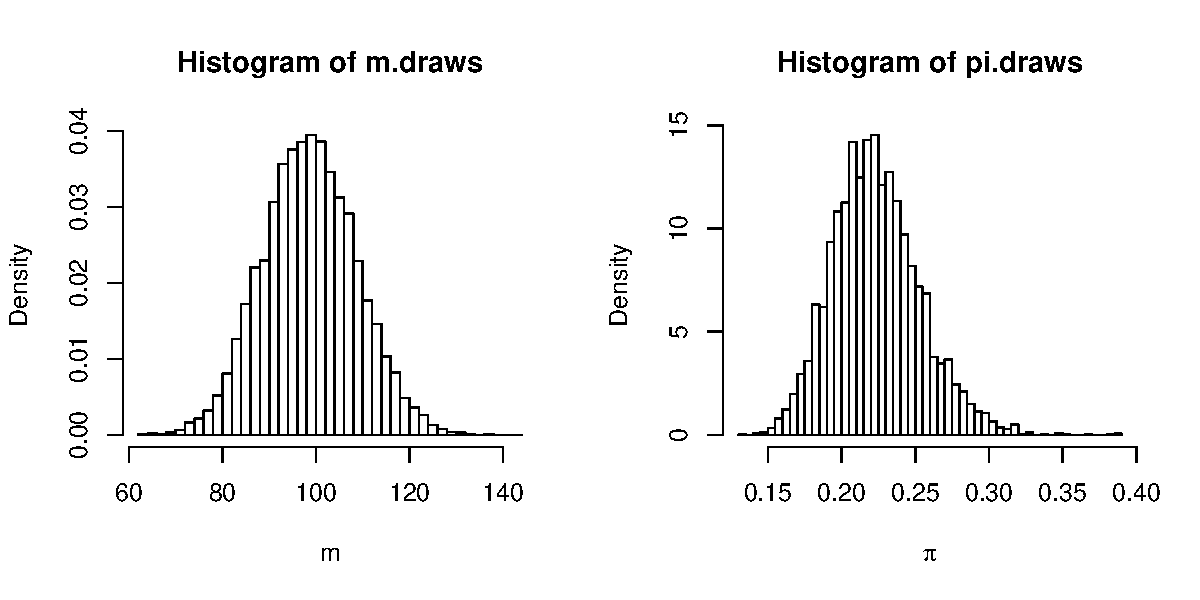
\includegraphics[width=\linewidth]{figure/converdiags-1} 

\end{knitrout}

\item disads

\item The hierarchical version of the model puts priors on $\lambda$ and priors on parameters of a $Beta(\alpha, \beta)$ distribution. I chose to put priors on the prior mean, $\eta = \frac{\alpha}{\alpha+\beta}$ and the somewhat approximate prior standard deviation, $\sigma = \sqrt{\frac{1}{\alpha + \beta}}$, kind of like what we did in the Beta-Binomial example with the stomach cancer data.
\begin{align*}
y_i &\sim Bin(m, \pi) \\
\pi &\sim Beta(\frac{\eta}{\sigma^2}, \frac{1-\eta}{\sigma^2}) \\
\sigma &\sim Uniform(0, 100) \\
\eta &\sim Uniform(0, 1) \\
\lambda &\sim Uniform(0, 500)
\end{align*}

\item The JAGs code I used to obtain draws from the above model is shown below.

\begin{knitrout}\footnotesize
\definecolor{shadecolor}{rgb}{0.969, 0.969, 0.969}\color{fgcolor}\begin{kframe}
\begin{alltt}
\hlcom{##write model file first}
\hlkwd{cat}\hlstd{(}\hlstr{"
model
\{
for(i in 1:N)
\{
y[i] ~ dbin(pi, m)
\}

pi ~ dbeta(eta/sigma^2, (1-eta)/sigma^2)
eta ~ dunif(0, 1)
sigma ~ dunif(0, 100)

m ~ dpois(lambda)
lambda ~ dunif(0, 500)
\}"}\hlstd{,}
\hlkwc{file}\hlstd{=}\hlstr{"model1.jags"}\hlstd{)}
\end{alltt}
\end{kframe}
\end{knitrout}


\begin{knitrout}\footnotesize
\definecolor{shadecolor}{rgb}{0.969, 0.969, 0.969}\color{fgcolor}\begin{kframe}
\begin{alltt}
\hlcom{##jags call}
\hlkwd{library}\hlstd{(R2jags)}
\hlkwd{set.seed}\hlstd{(}\hlnum{52}\hlstd{)}


\hlstd{dental.data} \hlkwb{<-} \hlkwd{list}\hlstd{(}\hlkwc{N}\hlstd{=}\hlkwd{length}\hlstd{(y2.data),} \hlkwc{y}\hlstd{=y2.data)}

\hlstd{inits} \hlkwb{<-} \hlkwd{list}\hlstd{(}\hlkwd{list}\hlstd{(}\hlkwc{pi}\hlstd{=}\hlnum{0.4}\hlstd{,} \hlkwc{eta} \hlstd{=} \hlnum{.00003}\hlstd{,} \hlkwc{m} \hlstd{=} \hlnum{100}\hlstd{,} \hlkwc{lambda} \hlstd{=} \hlnum{500}\hlstd{,}
                   \hlkwc{sigma} \hlstd{=} \hlnum{1.20}\hlstd{),}
              \hlkwd{list}\hlstd{(}\hlkwc{pi}\hlstd{=}\hlnum{0.2}\hlstd{,} \hlkwc{eta} \hlstd{=} \hlnum{.00003}\hlstd{,} \hlkwc{m} \hlstd{=} \hlnum{50}\hlstd{,} \hlkwc{lambda} \hlstd{=} \hlnum{150}\hlstd{,}
                   \hlkwc{sigma} \hlstd{=} \hlnum{2.24}\hlstd{),}
              \hlkwd{list}\hlstd{(}\hlkwc{pi}\hlstd{=}\hlnum{0.4}\hlstd{,} \hlkwc{eta} \hlstd{=} \hlnum{.00003}\hlstd{,} \hlkwc{m} \hlstd{=} \hlnum{150}\hlstd{,} \hlkwc{lambda} \hlstd{=} \hlnum{300}\hlstd{,}
                   \hlkwc{sigma} \hlstd{=} \hlnum{1.58}\hlstd{))}
\hlstd{n.chain} \hlkwb{<-} \hlnum{3}

\hlcom{#warmup}
\hlstd{warmup.model1} \hlkwb{<-} \hlkwd{jags.model}\hlstd{(}\hlstr{"model1.jags"}\hlstd{,} \hlkwc{data}\hlstd{=dental.data,} \hlkwc{n.chains}\hlstd{=n.chain,} \hlkwc{inits}\hlstd{= inits,} \hlkwc{n.adapt}\hlstd{=}\hlnum{4000}\hlstd{,} \hlkwc{quiet}\hlstd{=}\hlnum{TRUE}\hlstd{)}

\hlcom{#parameters to save}
\hlstd{params} \hlkwb{<-} \hlkwd{c}\hlstd{(}\hlstr{"pi"}\hlstd{,} \hlstr{"eta"}\hlstd{,} \hlstr{"sigma"}\hlstd{,} \hlstr{"m"}\hlstd{,} \hlstr{"lambda"}\hlstd{)}

\hlstd{n.iter}\hlkwb{=}\hlnum{50000}
\hlcom{#running the model for real}
\hlstd{model1} \hlkwb{<-} \hlkwd{coda.samples}\hlstd{(warmup.model1, params,} \hlkwc{n.iter}\hlstd{=n.iter)}
\end{alltt}
\end{kframe}
\end{knitrout}

\item The plots below compare the posterior distributions for $\pi$ and $m$ obtained in part (f) to those from the hierarchical model. There is much more variability in the posterior draws for $m$ and $\pi$ in the hierarchical model compared to the model with fixed hyperparameters. I think this makes sense because when the hyperparameter values are approximated, the model does not incorporate uncertainty in these parameters. With such a small sample size, the additional source of uncertainty accounted for in the hierarchical model makes a big difference in the results.

\begin{knitrout}\footnotesize
\definecolor{shadecolor}{rgb}{0.969, 0.969, 0.969}\color{fgcolor}
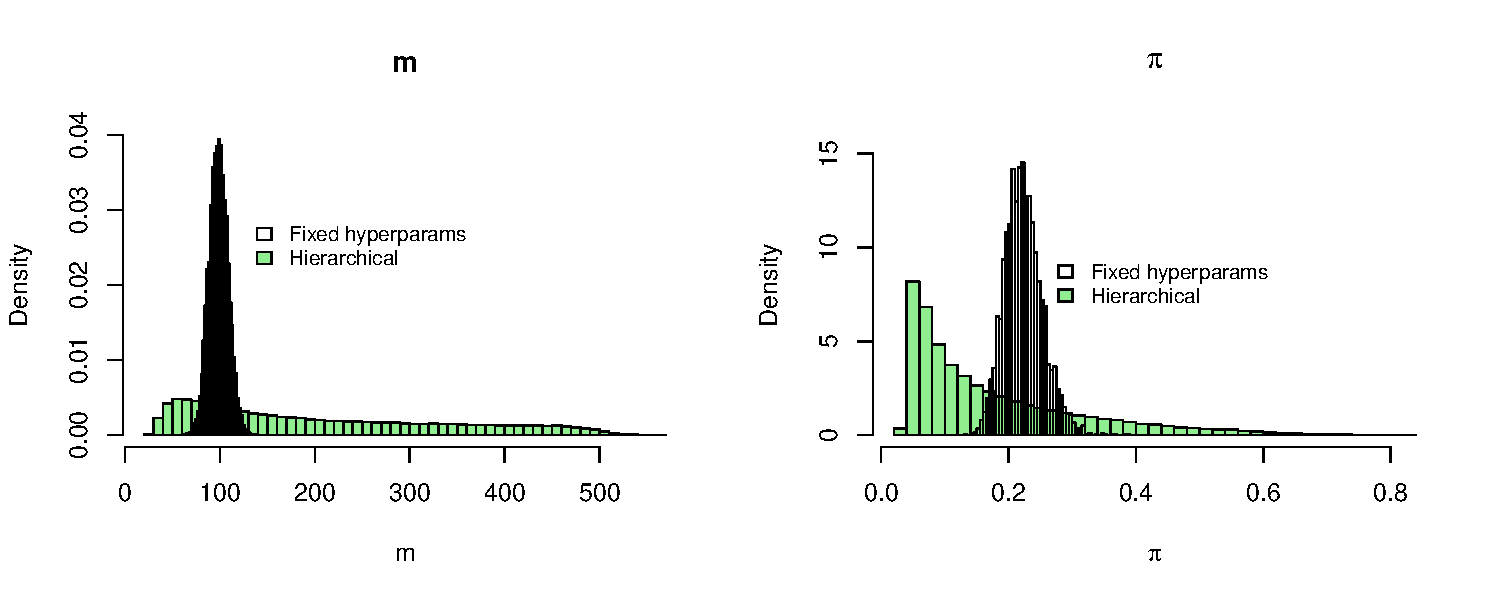
\includegraphics[width=\linewidth]{figure/jagsdrawscompare-1} 

\end{knitrout}

The posterior distributions of the hyperparameters are shown below, with the fixed values used in (e).

\begin{knitrout}\footnotesize
\definecolor{shadecolor}{rgb}{0.969, 0.969, 0.969}\color{fgcolor}
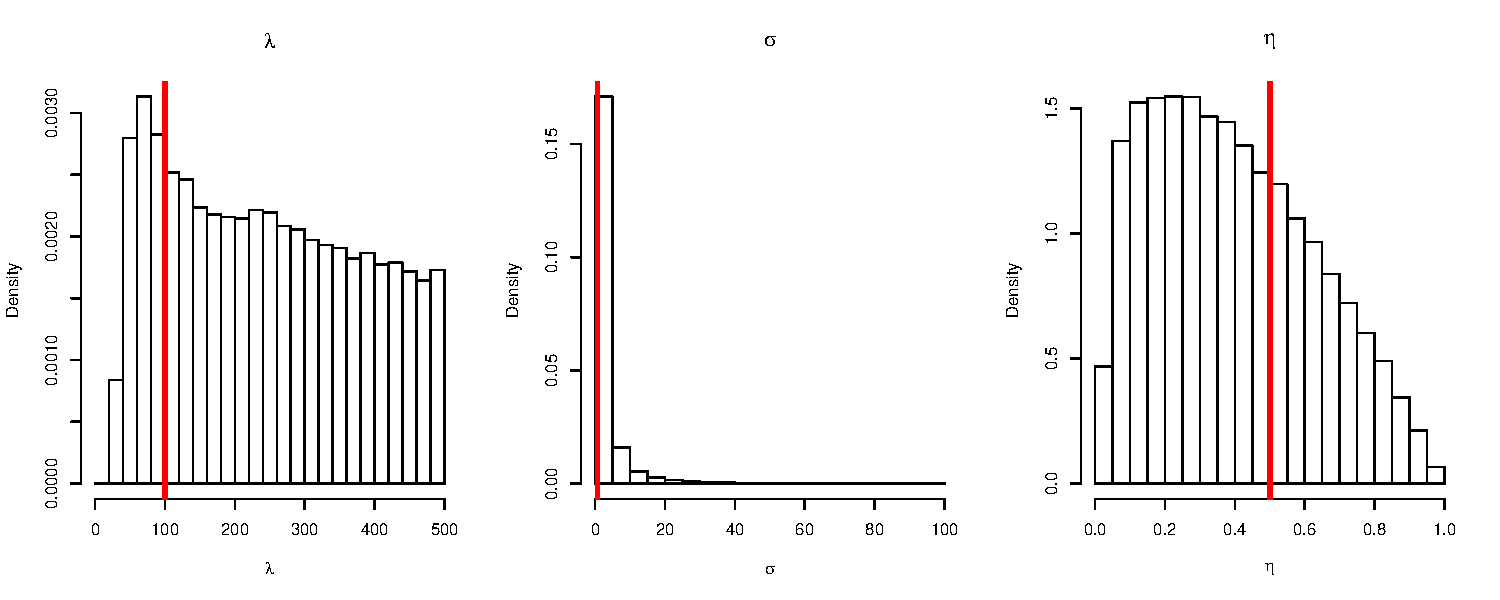
\includegraphics[width=\linewidth]{figure/jagshyperdraws-1} 

\end{knitrout}

\item

\end{enumerate}



\item \begin{enumerate}

\item The simple logistic regression model for estimating the dose-death relationship is as follows. I treat dose as a continuous predictor variable. The empirical probabilities of death at each dose as well as the fitted probabilities from the glm() model are shown on the plot below. The dose at which half of the frogs are estimated to die is $\frac{0.5 + 56.97}{78.29} = 0.734$ grams per ml. 
\begin{align*}
y_{ij} \sim& Bin(5, \pi_j) \\
logit(\pi_j) &= \alpha + \beta x_j
\end{align*}

\begin{center}
\begin{knitrout}\footnotesize
\definecolor{shadecolor}{rgb}{0.969, 0.969, 0.969}\color{fgcolor}\begin{kframe}


{\ttfamily\noindent\color{warningcolor}{\#\# Warning: glm.fit: fitted probabilities numerically 0 or 1 occurred}}\end{kframe}
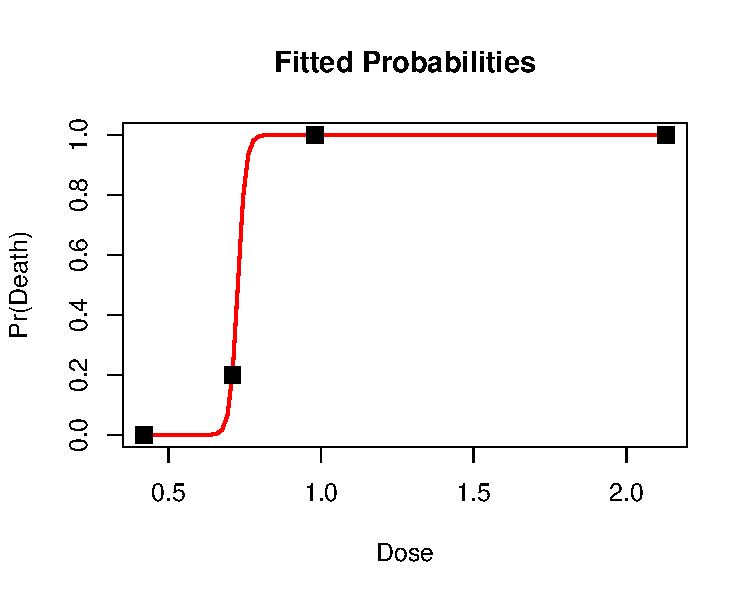
\includegraphics[width=.5\linewidth]{figure/glmmodel-1} 

\end{knitrout}
\end{center}

\item The model I will use to do the analysis in a Bayesian framework is shown below. 
\begin{align*}
y_{ij} &\sim Bern(logit^{-1}(\alpha + \beta x_j)) \\
\alpha &\propto 1 \\
\beta &\propto 1
\end{align*}

\item The model code is shown below.
\begin{knitrout}\footnotesize
\definecolor{shadecolor}{rgb}{0.969, 0.969, 0.969}\color{fgcolor}\begin{kframe}
\begin{alltt}
data \{
  int<lower=0> N;
  vector[N] x;
  int<lower=0,upper=1> y[N];
\}
parameters \{
  real alpha;
  real beta;
\}
model \{
  y ~ \hlkwd{bernoulli_logit}(alpha + beta * x);
\}
\end{alltt}
\end{kframe}
\end{knitrout}


\begin{knitrout}\footnotesize
\definecolor{shadecolor}{rgb}{0.969, 0.969, 0.969}\color{fgcolor}\begin{kframe}
\begin{alltt}
\hlkwd{require}\hlstd{(rstan)}
\hlkwd{set.seed}\hlstd{(}\hlnum{23}\hlstd{)}
\hlstd{data} \hlkwb{<-} \hlkwd{with}\hlstd{(frog.data,} \hlkwd{list}\hlstd{(}\hlkwc{y} \hlstd{= death,} \hlkwc{x} \hlstd{= dose,} \hlkwc{N} \hlstd{=} \hlkwd{length}\hlstd{(death)))}

\hlstd{model2} \hlkwb{<-} \hlkwd{stan_model}\hlstd{(}\hlkwc{file} \hlstd{=} \hlstr{"~/Documents/Stat532/exams/exam2/model2.stan"}\hlstd{,}
                     \hlkwc{model_name} \hlstd{=} \hlstr{"model2"}\hlstd{)}
\hlstd{samp2} \hlkwb{<-} \hlkwd{sampling}\hlstd{(model2,} \hlkwc{chains} \hlstd{=} \hlnum{4}\hlstd{,} \hlkwc{iter} \hlstd{=} \hlnum{2000}\hlstd{,} \hlkwc{data} \hlstd{= data)}
\end{alltt}
\end{kframe}
\end{knitrout}

\item The posterior draws for the y-intercept ($\alpha$) and the dose effect ($\beta$) are shown below. The red line indicates the estimate from the above generalized linear model.

\begin{knitrout}\footnotesize
\definecolor{shadecolor}{rgb}{0.969, 0.969, 0.969}\color{fgcolor}
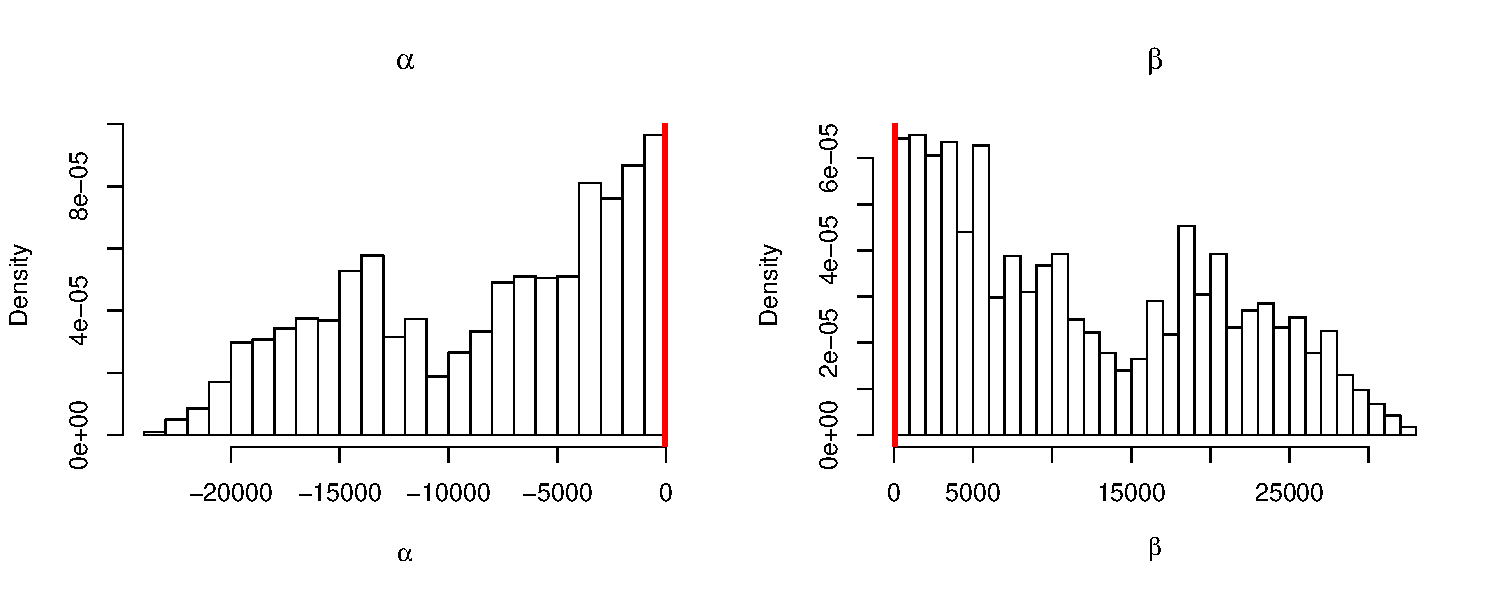
\includegraphics[width=\linewidth]{figure/compare-1} 

\end{knitrout}

\item Discuss and explain

\item The plots of the posterior draws for $\alpha$ and $\beta$ are shown below for the model with standardized dose as the predictor variable. The posterior draws for $\alpha$ have changed, but this is expected because $\alpha$ is now the log odds of death at the average dose. Standardizing dose does not appear to change inference about the effect of dose on the log odds of survival. Also, the efficiency of the sampler has not changed noticeably.



\begin{knitrout}\footnotesize
\definecolor{shadecolor}{rgb}{0.969, 0.969, 0.969}\color{fgcolor}
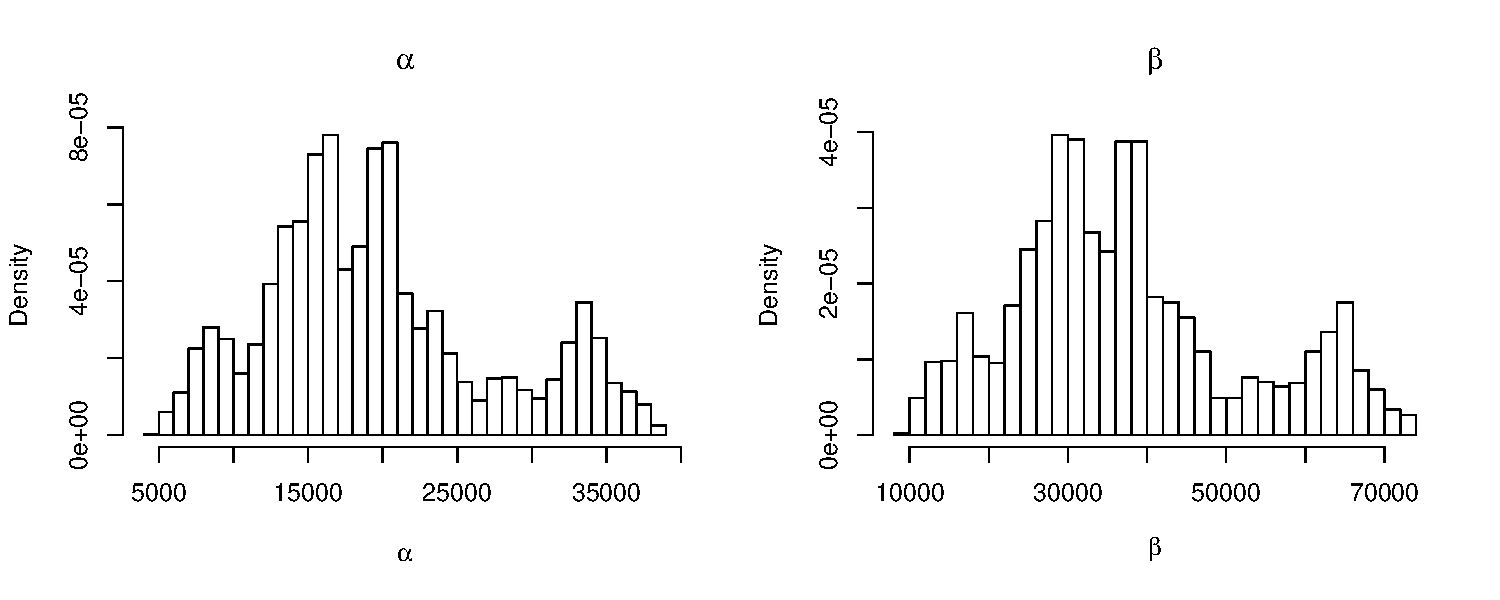
\includegraphics[width=\linewidth]{figure/stdcompare-1} 

\end{knitrout}


\end{enumerate}

\end{enumerate}

\end{document}
